% 原页四个定性图的轴、零点、渐近线与标号；曲线形状按正切模型示意重建。
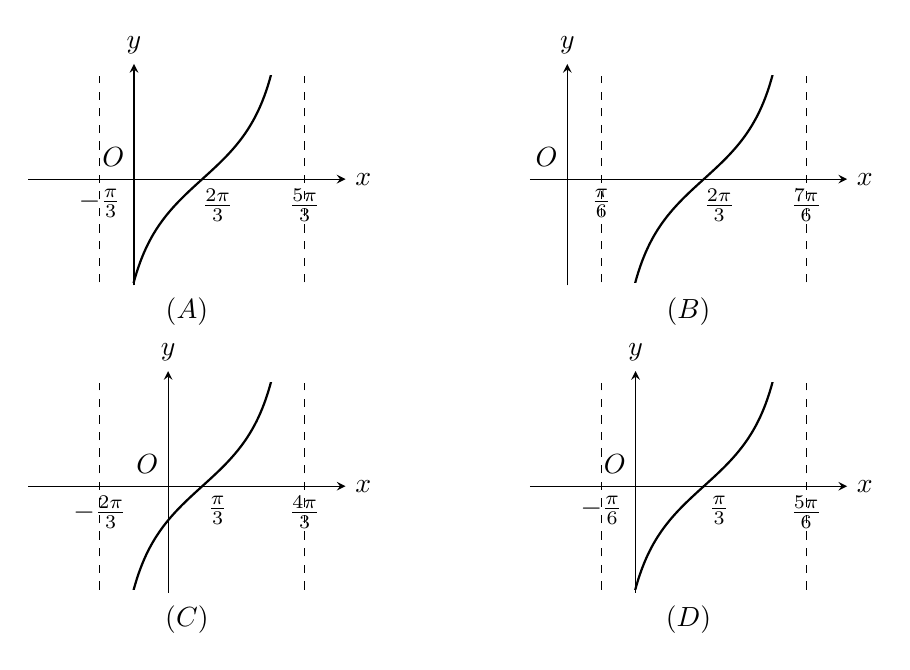
\begin{tikzpicture}[x=1.3cm,y=0.75cm,>=stealth]
\def\gkartsgraph#1#2#3#4#5{%
  \draw[->] (-1.7,0)--(1.4,0) node[right] {$x$};
  \draw[->] (#1,-1.8)--(#1,1.95) node[above] {$y$};
  \draw[dashed] (-1,-1.75)--(-1,1.75) (1,-1.75)--(1,1.75);
  \begin{scope}
    \clip (-1.7,-1.75) rectangle (1.4,1.75);
    \draw[thick,samples=100,domain=-0.92:0.92] plot (\x,{tan(90*\x)});
  \end{scope}
  \node[below] at (-1,0) {$#2$};
  \node[below] at (0.15,0) {$#3$};
  \node[below] at (1,0) {$#4$};
  \node[above left,yshift=1pt] at (#1,0) {$O$};
  \node at (-0.15,-2.25) {$(#5)$};
}
\begin{scope}
\gkartsgraph{-0.6667}{-\frac\pi3}{\frac{2\pi}3}{\frac{5\pi}3}{A}
\end{scope}
\begin{scope}[shift={(4.9,0)}]
\gkartsgraph{-1.3333}{\frac\pi6}{\frac{2\pi}3}{\frac{7\pi}6}{B}
\end{scope}
\begin{scope}[shift={(0,-5.2)}]
\gkartsgraph{-0.3333}{-\frac{2\pi}3}{\frac\pi3}{\frac{4\pi}3}{C}
\end{scope}
\begin{scope}[shift={(4.9,-5.2)}]
\gkartsgraph{-0.6667}{-\frac\pi6}{\frac\pi3}{\frac{5\pi}6}{D}
\end{scope}
\end{tikzpicture}
